\documentclass{article}

\usepackage{amsmath,amssymb,amsthm,graphicx,subfigure}

\pagestyle{myheadings}

\pdfpagewidth 8.5in
\pdfpageheight 11 in

\setlength\topmargin{0in}
\setlength\textheight{8.5in}
\setlength\textwidth{6.5in}
\setlength\oddsidemargin{0in}
\setlength\evensidemargin{0in}

\newcommand{\suchthat}{\ni}
\newcommand{\onlyif}{\Longleftrighttriangle}
\newcommand{\definedby}{\triangleq}
\newcommand{\union}{\bigcup}
\newcommand{\intersect}{\bigcap}
\newcommand{\where}{\mid}

\title{CIT 596 Homework 1}
\author{Steven Tomcavage\\stomcava@seas.upenn.edu}
\date{February 3, 2011}

\markboth{\hfill Steven Tomcavage }{\hfill Steven Tomcavage }

\begin{document}

\maketitle

\section{Exercise 1.4}

\subsection{Part e}

Create a DFA that accepts the language $\{\omega \where \omega \text{ starts
with an a and has at most one b}\}$.

\begin{figure}
	\centering
	\subfigure[A accepts $\{\omega \where \omega \text{ starts with an a}\}$] 
	{
		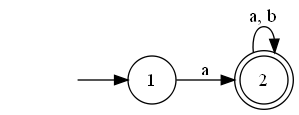
\includegraphics[height=1.0in]{1_4_e_a.png}
	}
	\subfigure[B accepts $\{\omega \where \omega \text{ has at most one b}\}$] 
	{
		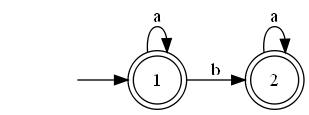
\includegraphics[height=1.0in]{1_4_e_b.png}
	}
	\subfigure[DFA that accepts AB] 
	{
		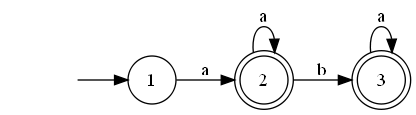
\includegraphics[height=1.0in]{1_4_e.png}
	}
	\caption{DFA for Exercise 1.4e}
\end{figure}

\subsection{Part f}

\subsection{Part g}

\section{Exercise 1.5}

\subsection{Part c}

\subsection{Part e}

\subsection{Part f}

\section{Exercise 1.6}

\subsection{Part c}

\subsection{Part e}

\subsection{Part g}

\subsection{Part i}

\subsection{Part j}

\section{}

\section{}

\end{document}
